\chapter{Daronpon: Datacenter Load Balancing Across Racks}
\label{daronpon:chap}

%\newcommand{\daronpon}[0]{Daronpon\xspace}
%\newcommand{\daronpon}{Daronpon}

\section{Introduction}
\label{daronpon:sec:intro}

To improve both performance and fault tolerance, datacenter
applications are provisioned to scale horizontally, with replicated
instances frequently spread across multiple racks of servers.  These
replicas must be carefully managed to meet strict service-level
objectives (SLOs) for both throughput and
latency~\cite{killer_microseconds,tail_at_scale}. These requirements
have birthed an architectural paradigm of highly replicated
microservices that can (nearly) arbitrarily fan out to deliver
ever-higher throughput, and whose functionality is scoped to provide
microsecond-timescale responses with low latency even in the tail.

Realizing this design pattern in practice poses multiple engineering
challenges, however.  Microsecond-timescale services must be resilient
to low-level system and network perturbations and short-lived
congestion events to achieve consistent
performance~\cite{facebook_microburst}.  These events arise within the
operating system, runtime, and application software as well as due to
network-level incast events, where many clients send to a
common destination server, causing in-network buffering and
substantial queuing delays~\cite{facebook_memcache}.  Moreover, the
potential impact of these so-called ``microbursts'' increases with
network bandwidth.  Large bursts can lead to packet drops and
necessitate end-to-end retransmissions.

Experience shows that a responsive and effective load-balancing
strategy is key to managing overall service latency.  Given the
ultra-low service times of many modern datacenter services, end-to-end
approaches driven by the clients and servers themselves are unlikely
to meet demands, as many component services (i.e., computation) times
are smaller than datacenter-wide network latencies. Instead, we focus
on in-network load balancing techniques carried out by network
switches or middle boxes---often generally referred to as
\textit{dispatchers}.  Recent work has shown the benefits of load balancing
with a server rack, for example R2P2~\cite{r2p2} and
Racksched~\cite{racksched}.  These approaches take into account server
load balancing, building upon prior approaches to core scheduling in
individual servers~\cite{IX,shinjuku,shenango,seda}. Further,
Vargaftik et al.~\cite{lsq} show that, for the multiple-dispatcher
environments that we target, a stable and highly efficient load
balancing approach is possible through a carefully controlled exchange
of status updates between servers and dispatchers.

We present \daronpon, an inter-rack load balancer targeted to network
services with sub-RTT service times.  \daronpon periodically
exchanges service-load information between dispatchers, either through
explicit gossip messages or piggybacked onto redirected application
requests.  We employ a logarithmic threshold approach to minimize
the network overhead of state-exchange messages while ensuring that
application requests are forwarded to replicas with good performance.
Our system decreases the 99th-percentile tail latency by up to a
factor of two over random replica selection across a variety of
workloads, enables scaling across heterogeneous server
configurations, and provides performance gains for service times as
low as two microseconds.
%
\footnote{
Services are assumed to be replicated throughout Chapter~\ref{daronpon:chap}, thus
replica and services are used interchangeable.}

% \TODO{Add a footnote saying replica and services are used interchangeable since all services are assumed to be replicated in this chapter.}

\section{Background}
\label{daronpon:sec:background}

%\textbf{Data Center Replication:}

Modern datacenter applications are
replicated~\cite{rocksdb,memcached,mongodb} to provide fault
tolerance, scalability and flexible response to load
fluctuations. Often, individual application components are replicated
on the order of three times for fault tolerance. In the case of
sharding for scalability, however, the number of replicas can be many
orders of magnitude higher and even grow
dynamically~\cite{facebook_shard,google_slicer,microsoft_service_fabric}
as needed to service demand.

\subsection{Datacenter load balancing}
%%
Traditional application or \textit{layer-4} load balancers operate across
the set of back-end services and maintain connection consistency for
long-lived flows. They are generally implemented in software using
commodity servers~\cite{cheetah, maglev, beamer, ananta}, although
some have explored using switches with hardware support~\cite{duet,
  silkroad}.  While effective at responding to end-host-driven load
imbalances, they are ill-positioned to address transient
variations in service times.

Conversely, conventional \textit{layer-3} load-balancing techniques focus on
dispersing traffic load in the network, and do not address server
imbalance.  For example, equal-cost multi-path routing (ECMP) load
balances flows using a hash of their 5-tuple. ECMP is widely deployed
due to the benefits it gains from average-case statistical
multiplexing.  It is well known, however, to cause load imbalance due
to hash collisions and when links fail.  A variety of improvements to
ECMP have been proposed, many using the concept of
flowlets~\cite{conga, clove, HULA, letitflow}: a group of packets
within the same flow separated from others by a large enough time
interval. Other schemes load balance per
packet~\cite{drill,flowbender,hermes}. Each of these in-network
techniques are complementary to our work, as they load balance
exclusively based on the state of the network and not the end-host
applications.

\subsection{Microsecond timescales}

Despite practitioners' attempts to spread demand evenly across both
servers and network fabrics~\cite{facebook:sigcomm15}, a certain
degree of variability is inevitable.  Indeed, as links speeds of 100 and
400-Gbps become the norm, hosts and switches can experience
significant traffic bursts over short periods of time. These bursts,
while lasting only a few microseconds, can cause congestion, lead to
increased jitter, and result in packet
drops~\cite{facebook_microburst}. As a concrete example, a switch with
64~MB of packet memory will overflow in 1.9~ms at
100~Gbps~\cite{tofino2} under incast scenarios.  While these events
originate in the network, the effect of that queuing cascades at the
application. Congestion impacts performance directly as batches of
requests are delivered in very short time periods.  Existing
end-to-end techniques struggle to react to microbursts effectively as
the durations of the microbursts are shorter than the network RTT
which bounds the response time of any end-host approach.

%\emph{Rack-scale load balancing:}

\daronpon\ targets microsecond-timescale services which
do not involve long-lived connections.
%Maintaining connections for
%microsecond timescale load balancing wastes precious resource on
%switches. \daronpon\ is
(We support any request/response service on top of a connection-less
transport or one with migration ability~\cite{crab,quic}.)  Techniques
for dispatching such microsecond-duration requests within an end-host
operating system have been explored recently~\cite{IX, shinjuku, snap,
  shenango, zygos}.  These end-host-based approaches use load-aware
schedulers to direct requests to CPU cores and to quickly rebalance
those allocations.  Extensions to these techniques demonstrate similar
scheduling performance at the scope of a entire server
racks~\cite{r2p2, racksched}. These efforts make use of programmable
switches to track end-host load at the rate of millions of requests
per second~\cite{tofino2}. Both R2P2~\cite{r2p2} and
Racksched~\cite{racksched} are confined to services which operate
entirely within a single rack due to a single control point within the
ToR switch. This limits the applicability of these schemes for the
majority of replicated applications which are distributed throughout
the datacenter.

Researchers have also explored explicitly integrating different
replication techniques with programmable switching hardware to avoid
RTT delays, including chain replication~\cite{netchain},
Raft~\cite{hovercraft}, and Paxos~\cite{nopaxos}.  In-network
replication techniques have also been proposed to alleviate
read/write conflicts~\cite{harmonia} and
contention~\cite{pegasus}. 
%
\daronpon operates under the assumption
that replicas are interchangeable for all requests; our
techniques could be extended to support any of these protocols, however
\daronpon would require protocol-specific information to operate.

\section{Challenges}
\label{daronpon:sec:challenges}

Theoretically, optimal load balancing is attainable with centralized
algorithms~\cite{jsq_fcfs} that maintain full knowledge of the global
instantaneous system load.  
%
A proven-optimal algorithm, join-the-shortest-queue (JSQ), ensures requests experience minimal queuing delay.  
%
Unfortunately, centralization prevents cross-rack sharding and scale-out designs.  
%
In contrast, fully decentralized approaches (e.g. client-based power-of-two designs~\cite{power_of_2}) either require network-wide message round trips to measure load or rely on out-of-date information from previous response.
%
As the service time of requests approaches that of an RTT, 
both approaches provides little benefit on acquiring more up-to-date information.
% the cost of extra probing increases the latency of the request and consumes more link
% capacity (i.e two RTTs per request). 
%
Further, these approaches struggle to react quickly to congestion given these long network-wide round-trips. 
%
Load-balancing decisions made with information which has aged by at least an RTT cannot react to microburst events which occur on sub-RTT timescales.

\subsection{Microsecond load balancing at scale}

An ideal solution for microsecond load balancing at scale will therefore be
decentralized to avoid bottlenecks, designed to reduce probing overheads, and
designed to react nearly instantaneously to bursts.
Vargaftik et al.~\cite{lsq} demonstrated theoretically that distributed
load balancing for datacenter scale is possible. Their proposal, LSQ, has many
desirable properties such as a bounded measurement difference between true
server load and the load observed by a load balancer, which receives load
updates as messages using a variety of mechanisms~\cite{lsq}. 

We investigated via simulation an implementation of LSQ in which we
placed LSQ load balancers on core routers within a fat tree
network. Using core switches satisfies LSQ's theoretical assumptions
with regard to how each load balancer sees sever load by forcing all
packets through the core of the network to ensure that every request
is visible.  In this core-switch realization of LSQ, we find some
practical limitations.  The first of which is its (lack of) response
to microbursts. When requests target the same server, the available
bandwidth on the egress port of that server's associated top-of-rack
(ToR) switch is stressed, leading to drops~\cite{facebook_microburst}. These bursts
occur due to lack of coordination between core routers; they can be
prevented by making load-balancing decisions at the ToR instead.
%rather than at the core.

Hence, we propose to load balance on leaf ToRs directly. This
alteration has a variety of implications on LSQ's theoretical
approach. First, LSQ has approximate knowledge of all server
queues. By moving our load balancer to ToRs we lose instantaneous
knowledge of remote queues but gain up-to-date load information for
all the servers of a rack beneath a ToR.  
%
While this updated knowledge gives us tremendous insight into the state of that single
rack as shown in R2P2 and Racksched~\cite{r2p2, racksched}, it leaves the
dispatchers unaware to the load of services running on remote racks.
%%
A key challenge in this work is designing a ToR-based load-balancing
approach for datacenter scale by maintaining accurate estimations of
the load of other servers at remote ToRs in the absence of periodic updates. 
%on the data path (as is the case in LSQ).
%queue lengths

%ToRs also have the advantage of being general,
%regardless of the upper level data center topology (Fat-Tree,
%Expander, Jellyfish)
%%

%The largest problem with load balancing around microbursts is finding
%a suitable location at which to perform load balancing. Because
%congestion can happen throughout the network, and the events are on
%the order of an RTT. No single position is perfect. In this section we
%describe the trade offs of placing a load balancer at different
%positions throughout a datacenter network, and the challenges
%associated with keeping such as system synchronized and responsive at
%short timescales. Specifically we contrast end to end approaches using
%both clients and servers, then consider various in network locations
%within a fat-tree topology.


%\todo{rephrase Servers are the same as tors, but we need to inflate
%gossip messages, the link is more congested, and we are using end host
%processing}
%\textbf{Servers} could act as their own gatekeeper, rejecting or
%redirecting requests when they are overloaded.  This approach has
%multiple downsides.  First, it requires servers to efficiently monitor
%their own application load which requires additional compute and can
%be difficult to attain accurately. Various research projects have
%aimed to attain such information precisely, usually at the cost of
%additional processing cores~\cite{shenango,shinjuku_offload}. These
%approaches require that application developers tightly couple their
%programs with the runtime. In the case of off-the-shelf Linux, its
%networking stack has limited ability to provide precise
%application-level load information, such as number of outstanding
%requests for a particular service. Linux's I/O event polling
%%mechanism, {\em epoll}, operates on file descriptors level, and it
%doesn't provide efficient methods to peek into the number of requests
%under each file descriptor.  XDP~\cite{xdp} provides a fast and
%efficient way to handle application request packets within the kernel
%space but it requires corresponding eBPF program to be injected into
%the kernel.  Second, TOR-server links are where most micro-bursts and
%packet drops occur ~\cite{jupiter-rising,facebook_microburst}
%throughout the datacenter.  We want to avoid sending any additional
%requests to servers that could worsen the condition of already
%stressed links.  

%%
%Additionally from a network perspective core switches are far from
%endhosts. Network conditions may vary on the south bound path towards
%the endhosts. Each of the core switches must act independently on their
%local knowledge of each replica, which is invariably incomplete. For
%instance two core switches could target many request to the same
%endhost without sharing their load balancing decisions with each other
%leading to incast. This leads to the fundamental problem of making a
%\textit{predictive} decision about endhost load. Aggregate suffer
%from a similar problem at a pod granularity.

\subsection{Load knowledge}

At datacenter scale, any centralized load balancer is proned to be a performance
bottleneck. 
%
This is true not only in terms of traffic, but also in terms of the per-application state that the load balancer needs to track. 
%
In the absence of centralized knowledge, load information must
be distributed among load balancers. 
%
While the potential benefit of making decisions locally with even out-of-date information is substantial, the hazards of load balancing in ignorance are
documented in the literature~\cite{dahlin_stale_info,mitzenmacher_old_info}. 
%
The question of how to efficiently disseminate timely state information in
practice remains open.

Updates issued periodically between load balancers leads to a
predictable overhead in terms of bandwidth and number of messages, but
admits (potentially unbounded) errors in the estimates at remote load
balancers. 
%
Assuming that events arrive with a Poisson or exponential
distribution, many events can occur between load information message
exchanges.  
%
Alternatively, state updates could be disseminated in relation to the request rate, with updates being issued for every request or perhaps some fraction of the total number of requests. 
%
This too suffers as the number of messages issued during bursts of requests
can cause an increase in update traffic at the worst possible
time. 
%
The choice of how to disseminate load in a way that provides
up-to-date information in a non-obstructive way is crucial to \daronpon's design.

%\begin{figure}[t]
%  \centering
%    \includegraphics[width=0.45\textwidth]{fig/no_gossip.jpg}
%    \centering
%    \caption{\todo{Percentage improvement in load balancing decisions given
%%    50us load updates}}
%    \label{fig:no_gossip}
%\end{figure}

\subsection{Stale information}

The following experiments show that the frequency at which load is updated has a
significant effect on the quality of the decisions. 
%
However, there is a trade-off in terms of traffic overheads to keeping information up 
to date. 
%
As the number of services increases, so too does the number of messages needed to
keep the information fresh. 

Given imperfect, or stale, information about remote servers, the
question becomes: \textit{when is redirecting requests a good course of action}? 
%  
We submit that given reasonably predictable, but
potentially eccentric, request patterns, the correct course of action
is to act conservatively when conditions are manageable, and to react
quickly and decisively when request loads spike, i.e., in microburst
scenarios.  
%
These constraints dictate a compromise between inflating traffic and making sub-optimal decisions with poor information.

\subsection{Information traffic reduction} 

Determining how often and when to send load information requires
careful consideration. If an update were to be propagated for every
request, that would be ideal from a decisions making perspective, but
the overall number of messages sent could inflate by the total
replication factor (2$\times$ or 3$\times$ in many cases).  Such
overheads are unacceptable for systems with requests in the thousands
or millions of requests per second as the cost of the information
quickly surmounts the goodput traffic. A key challenge in designing a
distributed in-network load balancer approach is to identify the most
critical information to send which ideally only produces a small
overhead in terms of state exchange messages.

%\subsection{Predictability}

Network operators generally want predictable behavior within their networks.
Given that distributed load balancing requires information to be spread, it
raises the risk of adding unpredictability to the network, specifically in
terms of overhead. An ideal load-balancing strategy would spread information
efficiently while allowing operators to set an overhead budget in terms of
bandwidth or messages which would correlate to a comparable increase in
performance. Predictability is highly important in heterogeneous systems where
multiple applications require guarantees about their apportioned network share.

\subsection{Heterogeneous rack configurations}

At datacenter scale the configuration for any application may vary wildly.
Individual service replicas may be co-located with resource-hungry applications.
Due to configuration differences applications might have varying processing
powers. Many applications are placed in VMs which execute on differently
powered hardware. Indeed, in the datacenter there is no guarantee that any set
of replicas is equally provisioned. Therefore, any load-balancing strategy must
take into account this heterogeneity and apportion requests in response to the
real processing rate.

\section{Daronpon design}
\label{darapon:sec:design}

The \daronpon design resides within the ToR at each rack and is designed to
track server load by counting the number of outstanding requests for each
service running on that rack. Figure~\ref{fig:racks} illustrates the role that
ToRs play in our load balancing scheme.  When a request arrives at a ToR it
makes a load balancing decision. It either \textit{Admits} the request, or it
\textit{Redirects} it to another replica. The choice to either admit or
redirect is subject to the local load the service is currently experiencing
under the ToR (as understood by \daronpon), and an estimation of the load
each replica has on remote ToRs. 

%If a request is admitted the ToR increments it's
%load counter for that service. Once the server complete the request
%and the response from that service passes back through the ToR the
%load counter is decremented. Each TOR has a perfect count of the
%number of outstanding requests underneath it (assuming reliable RPC)
%which it can use to request count of services running on remote racks
%are sent periodically which give ToRs approximate knowledge of their
%load.  Using this information ToRs make the decision to \textit{Admit}
%or \textit{Redirect} a request when it arrives. 

A ToR can only directly keep an up-to-date counter for the services running in
its rack. To make good load balancing decisions, fresh knowledge, and more
importantly knowledge of bursty behavior, is necessary.  Determining the
mechanisms for disseminating this load information is non-trivial.

We designed and tested a variety of different options for disseminating load
information in simulation and on an Amazon Web Services (AWS) testbed.  One
design gossiped load information periodically based on wall clock time, and
another gossiped on a per-request basis. Our results in simulation and on our
test setup demonstrate that both of these techniques require extremely high
overheads in terms of messages sent.  For example, our best results with
periodic message exchanges required updates polled every 25us. This resulted in
over a 2x overhead in terms of messages. Most of the information spread in this
case was redundant, and does not aid in mitigating bursts.  Further, it adds
congestion to the network, which reduces the maximum throughput, especially
during bursts, which is the opposite of our goal. An ideal load dissemination
design would quickly react to bursts while simultaneously generating little
overhead during burst events.

\daronpon consists of two distinct but complementary messaging
mechanisms.  
%
The first mechanism is logarithmic gossip that guarantees the reactive spread of load information when bursts occur, 
while generating little overhead otherwise.  
%
The second one is opportunistic piggybacking that spreads load information between ToRs when requests are
redirected. 
%
We find in our evaluation that our log gossip approach prevents large queue build-ups, while our piggyback approach greatly reduces latency in the common case.  
%
%These results are outlined in detail later in this paper.

\begin{figure}[ht]
  \centering
    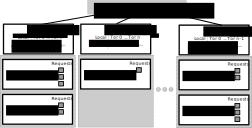
\includegraphics[width=0.8\textwidth]{./figure/daronpon/racks.pdf}
    \caption{High-level overview of \daronpon. Each ToR tracks
    outstanding request for services running in its rack, and
    maintains approximate counters for remote ToRs hosting shared
    replicated services.} 

  \label{fig:racks}
\end{figure}

%\subsection{Gossip Periods}
%\begin{figure}[ht]
%  \centering
%    \includegraphics[width=0.45\textwidth]{fig/diffgossip.pdf}
%    \centering
%    \caption{Different gossip periods from 1\/2 RTT to 16 RTTs. Using constant service time 25 us} 
%  \label{fig:diffgossip}
%\end{figure}

%Information about remote load counters is the key factor in making
%redirection decisions. Out-of-date load information is of low utility
%over time as its accuracy decreases. Therefore, the
%load gossip period has a remarkable effect on the overall performance.

%We tested the effect by running different gossip periods.
%After each run the period of gossip messages is doubled, starting at 25 us. 
%Figure~\ref{fig:diffgossip} shows the resulting
%trend when our servers are stressed at 30k request per second. 
%While doubling the gossip period, we can see 
%a linear performance degradation on 95th, 99th, and 99.9th percentiles latency
%starting at 100us, i.e. 1 RTT.
%The 50th, 95th, 99th, and 99.9th percentiles latency increase
%4.4\%, 26.9\%, 42.7\%, 58.3\% with 32x gossip periods. 

%%
%A marginal benefit is found at any gossip periods as a local redirections
%require a queue depths of 1 or greater, and even with poor information
%the probability of a redirected request landing at a less stressed
%server is sufficient enough for a performance benefit. 



% \sg{The aggregate number of gossip messages grows exponentially with the number
% of services running under each TOR. We should consider pointing out
% some mechanisms which might amortize the cost of these messages.}

% \begin{figure}[t]
%   \centering
%     \includegraphics[width=0.45\textwidth]{fig/load_spread.pdf}
%     \centering
%     \caption{ Request latency response to gossip message frequency
%     with servers loaded at 70\%. Exponential increases in frequency
%     lead to linear increase in performance. ~\todo{make off values
%     line up with ~\ref{fig:delta}} ~\todo{average over more runs, this
%     is taken over 10}.
% }
%     \label{fig:load_spread}
% \end{figure}

%\subsection{Load Delta}
%\begin{figure}[ht]
%  \centering
%    \includegraphics[width=0.45\textwidth]{fig/diffdelta.pdf}
%    \centering
%    \caption{Different load delta values to avoid aggressive redirection. Using constant service time 25 us} 
%  \label{fig:diffdelta}
%\end{figure}

%Figure~\ref{fig:diffdelta} shows microbenchmark results 
%of requests latency varies across delta values. 
%Applying ToR redirection with small delta values improves performance. 
%However, larger delta values avoid aggressive redirections but they hurt
%the performance by missing redirection with potential benefits.
%We can see the tail latency substantially increased after delta value of 10 under 
%a 35 KRPS request rate.
%The 50th, 95th, 99th, and 99.9th percentiles latency increase 
%23.0\%, 20.9\%, 13.3\%, and 12.5\% when delta value increase from 10 to 80.

%\begin{figure}[ht]
%  \centering
%    \includegraphics[width=0.45\textwidth]{fig/diffdelta0to10.pdf}
%    \centering
%    \caption{Zoom-in view of delta values from 0 to 10. Using constant service time 25 us} 
%  \label{fig:diffdelta0to10}
%\end{figure}

%As shown in Figure~\ref{fig:diffdelta0to10} increasing delta values
%from 0 to 10, we saw a smaller but observable increase on latency.  We
%observed 22.0\%, 19.9\%, 14.2\% increase on the 50th, 95th, and 99th
%percentiles latency.  The increase on 95th, and 99th percentiles
%latency starts at delta value = 5.

%We saw a local minimum of request latency at delta value 2 and 3 at medium request rate 30kRPS.
%Using delta=2 gives us 7.1\%, 8.2\%, 7.8\%, and 7.1\% improvements on
%on 50th, 95th, 99th percentiles, and 99.9th percentiles. Throughout
%our experiments we use a delta value of two as our local optimum.


%\todo{Load delta can be used as a way to reduce the total number of
%packet redirections. Should we choose to add redirections to the cost
%of our algorithm we want to show how using a load delta can decrease
%that}

\subsection{Microbursts}

Figure~\ref{fig:microburst} (top) shows an example of a microburst. In this
case, requests are issued at a Poisson arrival rate by multiple clients.  The
peaks show outstanding requests from the perspective of a ToR instrumented to
track request counts. In this case, when requests queue, that queue grows
without bound, even though other replicated services are available to process
this influx of requests. This has a dramatic impact on the tail latency of the
requests in the burst, and also the overall mean request time. A typical
request incurs longer wait times due to decreased overall system throughput.

In Figure~\ref{fig:microburst} (bottom) the queue builds up with our
logarithmic gossip mechanism enabled. Each \textit{red X's} on the chart
represents a point at which the load on the server is gossiped.  Note that when
peaks occur, and a gossip is sent, the load is quickly spread to other servers.
This increases overall system throughput and decreases tail latency. This
strategy, however, is not perfect. At low load the benefit of redirecting
requests is minimal. For example, when the number of outstanding requests is
just one or two above a remote service, and so redirection reduces overall
performance.

The age of the gossiped information complicates the act of redirecting. The
remote information on remote hosts is at least a few microseconds out of date.
Given the few microsecond budget our requests have to begin with, the benefit
of redirection quickly evaporates if even a few requests arrive from the point
in time at which the load information is sent.  This leads to unnecessary
redirections and high overheads in terms of gossip messages which do not
ultimately deliver useful information. This overhead can be mitigated by adding
a threshold which prevents gossip messages from being sent until the number of
outstanding requests has exceeded a given threshold.  Our proposed log gossip
technique for curtailing this overhead is described in the following section.

%Gossip messages consume and packet processing time.  Therefore their
%frequency must be chosen with care as to not introduce significant
%variance into the system. The majority of data center packet drops
%occur on south facing ToR egress to the host.~\cite{jupiter-rising},
%our approach only increases bandwidth above the ToRs which allows for
%a higher gossip bandwidth budget prior to it causing significant
%interference. Gossip messages are small, (approximately
%64 bytes depending on the number of services), which reduces aggregate
%bandwidth consumption.

%Our testbed results use gossip messages as
%frequently as 10us without any noticeable interference on 40Gbps
%networks. As network speeds increase we anticipate that the available
%bandwidth for background traffic which improves the performance of
%running services will increase.


\begin{figure}[t]
  \centering
    \includegraphics[width=0.80\textwidth]{./figure/daronpon/burst.pdf}
    \centering

    \caption{Microburst with no mitigation (top) vs. with
    logarithmic gossip load balancing enabled (bottom)}

  \label{fig:microburst}
\end{figure}

\subsection{Packet flow}

The \daronpon\ load balancers are stateful and act per request.
Figure~\ref{fig:load_balancer} provides a high level message flow diagram of
this system.  When requests arrive, \daronpon executes the admission
protocol. Requests are admitted only if the local service has the minimum
observable global load. A load tracker keeps counters for each global service.
Local counters are up-to-date, while remote counters are learned via gossip and
piggyback messages.  When a request is admitted, the ToR increments its load
counter corresponding to that service.  When a response passes back through the
ToR, that service has its local counter decremented.  If, when a request
arrives, the local load of a service is not the global minimum, the request is
redirected. The redirected request is then sent to the service with the lowest
load, based on the ToRs' local load tracker (see
Section~\ref{daronpon:sec:design:piggyback}).  Redirected requests have load information
attached to them. The attached load consists of request counters for the
intersection of services the ToRs share.  Therefore, the overhead per
redirected request is variable as per the systems' configuration.

Increments and decrements in local load are tracked by a gossip monitor (see
Section~\ref{darapon:sec:design:gossip}). The job of the gossip monitor is two-fold. First,
it identifies bursts. When load spikes the monitor broadcasts gossip messages
to let other ToRs know it is experiencing high load. Second, it identifies
valleys. Load balancing schemes which use potentially stale information are
known to exhibit herding behavior, a condition which leads to sub-optimal
queuing behavior~\cite{dahlin_stale_info,mitzenmacher_old_info}. When load
drops sharply, gossip messages are also generated to announce that a service
has spare processing capacity.

\begin{figure}[t]
  \centering
    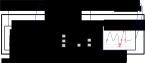
\includegraphics[width=0.80\textwidth]{./figure/daronpon/load_balancer.pdf}
    \centering

    \caption{ %% 
        %%
        Key functionality and message flow of \daronpon.
        Incoming requests are either admitted or redirected.
        Redirected requests spread load information via piggyback.
        Load is updated upon admission, and response.  Gossip messages
        are issues when load breaks a logarithmic threshold.}

  \label{fig:load_balancer}
\end{figure}

\subsection{Logarithmic Gossip}
\label{darapon:sec:design:gossip}

\begin{figure}[t]
  \centering
    \includegraphics[width=0.90\textwidth]{./figure/daronpon/log_thresh.pdf}
    \centering
    \caption{The percentage of gossip messages generated by a
    logarithmic gossip mechanism as a percentage of overall traffic.
    Collected from runs of 96 KRPS.} 
  \label{fig:log_thresh}
\end{figure}

\daronpon generates gossip messages aiming to reacting quickly to bursts while consuming little overhead in terms of additional messages.  
%
In an earlier design, ToRs gossiped load information every 25 $\mu$s. 
%
This logarithmic gossip approach has the advantage of providing highly updated load information, but it incurred scalability bottlenecks as the number of ToR increased, since the 25 $\mu$s gossip contends with request goodput for link bandwidth.

To compress the number of messages, \daronpon's gossip messages are sent
on exponential changes in load. 
%
\daronpon uses powers of two as the interval. 
%
\daronpon chooses two for its ease of computation requiring only bit shift operations because no commodity programmable switch, to our knowledge, is able to compute floating point arithmetic~\cite{challenging_programable}.
%both for its effectiveness in practice and 

Each step increases the bounds in which server load can fluctuate
prior to a gossip message being issued. 
%
For instance, if the load were to
increase from 1 to 2, a gossip message would be broadcast to all other servers
with the replicated service that crossed this threshold.
%
In this message, load information for all other shared services is added. When the boundary of two is crossed, and the value of two is sent, this ToR will not issue another gossip message until the load on the service rises by a power of two to four, or falls back down by a power of two to one.

%%
%% Sorting microbursts by size
%%
Logarithmic gossip has several benefits. 
%
First, it sorts microbursts by magnitude without adding significant packet overhead. Given that small fluctuations may occur at rapid pace, it is important to give priority to bursts with larger magnitudes.
%
% Other methods of achieving this goal such as piggybacking can lead to stale information, which has significant differences to ground-truth values, even when a server is experiencing very high load.


%%
%% Reduces congestion when bandwidth is needed
%%
Second, logarithmic gossip reduces the number of gossip messages sent during 
bursts, which reduces the overall strain on the system when resources
are at their tightest. 
%
This is an issue with gossip strategies that operate periodically (e.g. at preordained wall clock times) or are issued at some constant ratio
to requests (e.g gossip every 5 requests). 
%
When request rates are low, gossip messages are automatically sent with a higher frequency per number of requests which allows for better decision-making at lower
request rates.
%%
%%Aggregation of requets
%%
ToRs have the advantage of being an aggregator for the load of an
entire rack. 
%
Were we to implement our solution on end hosts, each host
would need to gossip its load to every other host. 
%
Using ToRs, the load of each server in a rack is known explicitly and is gossiped in its entirety, assuming the rack sees both requests and the associated
responses.

%%
%% Fast reaction
%%
Other approaches which use load information collected from end hosts
themselves suffer from additional delays in responding to load spikes,
as the knowledge of load must be transmitted to the balancer before it
can react. \daronpon's logarithmic gossip mechanism reacts to load as soon as a request is admitted. 
%
This allows for precise load balancing decisions to be made at sub-RTT time scales. 
%%
For instance, in a Fat-Tree with two ToRs connected by a single
aggregate switch, the distance traveled by load updates is halved in
comparisons to a host based solutions (e.g. Tor-Agg-Tor vs
Host-Tor-Agg-Tor-Host). This approach is not limited to Fat-trees,
as many networks use ToRs, however our ToR-based approach always results
in two hops less than an host based approach.

%% %Approximate measure of load, but fast react %
\daronpon's logarithmic gossip estimates server load on the ToR with counters instead of  requiring precise and up-to-date measures of load on the host, which we can
only get with precise application level knowledge and host control, 
%
This imposes lower tracking overhead, and performs nearly as well as highly tuned approaches which report server load directly~\cite[Figure. 15 (proactive)]{racksched}.
%%
%% Threshold
%%
This algorithm decreases the number of gossip messages
significantly, and can be greatly improved by carefully considering a
lower bound at which to disable the mechanism entirely.
For example, setting a lower threshold such as $t$ implies that below an outstanding request count of $t$ a ToR will not gossip information.
%
The threshold is determined by an exponential weighted moving average and a floor value that the threshold does not go beneath it.

Figure~\ref{fig:log_thresh} shows the percentage of messages gossiped relative
to the requests processed for different threshold values.  Note that the
default values of 0 and 1 have an overhead of around 30\% of the request rate.
Redirections of requests at these levels of outstanding request sees little
benefit in terms of performance as at any reasonably high request rate, the
depth of remote queues have changed since the remote data was received making
the choice stale. 
%
By increasing the threshold to four, the overhead in gossip
messages is reduced by a factor of ten down to around 2\% when our system is
around 70\% saturation. 
%
This suggests four is a good floor value for the gossip threshold setting.
%
See Section~\ref{sec:service_time} for a comprehensive
evaluation of gossip overhead. Increasing the gossip threshold beyond four
significantly reduces overhead down to around 0.02\%, however this comes at the
cost of only identifying bursts of size eight and greater which significantly
effects our reductions in 99th percentile tail latencies.

%%
%% Staleness
%%
Logarithmic gossip, however, provides no liveness
guarantees to the freshness of the load information announced despite all the aforementioned benefits. 
%
For instance, a server which maintains an outstanding number
of requests between 4 and 16 for $n$ requests will not issue a gossip
until either threshold is crossed. While this is unlikely in practice
due to the small range and short duration of requests, there is no
guarantee. This can become an issue for extended periods of load when
the number of outstanding requests is deep (e.g. 128 to 512).

\subsection{Piggyback}

\label{daronpon:sec:design:piggyback}
\begin{figure}[t]
  \centering
    \includegraphics[width=0.90\textwidth]{./figure/daronpon/breakdown.pdf}
    \centering
    \caption{Performance breakdown of gossip and piggyback mechanisms.
    Lower values are better.} 
  \label{fig:breakdown}
\end{figure}

Beyond using logarithmic gossip, the redirect requests also able to propagate load information by making load information riding with these requests heading to remote ToRs.  
% Using logarithmic intervals for gossip messages, we can identify and
% mitigate bursts.  
%
% Logarithmic gossip propagates load information, when the intervals are met, to remote ToRs, but the opportunities provided by redirected requests is untapped. 
% While this is advantageous in general, there is still
% additional performance to be gained.  
%
With gossip enabled, the percentage of redirected requests is 22\%. 
%
Each of these redirected requests is sent from the redirected ToR to the receiving one, and therefore has the ability to report the load information on the ToR that performed the redirection.  
%
We refer to this method of attaching load information to
redirected requests as piggyback, and using redirection to spread information
provides significant advantages in the common case.
%
Piggybacking depends on a threshold called load delta indicating the difference 
between the load on local replica and the load information on remote replica.
%
Load delta determines the triggering of redirection and controls the aggressiveness of redirection.
%
It is determined by an exponential weighted moving average as a threshold to adapt for different workload patterns.

In contrast to the centralized approaches in both Racksched and
R2P2~\cite{racksched, r2p2} piggybacking information load on requests
is not a sufficient mechanism for learning about remote load. This is
because our load balancer is decentralized, which means that our load
balancers do not see load information updates from every request.
Unlike our logarithmic gossip mechanisms, it provides no guarantees
about its operational bounds. Using gossip messages exclusively
provides no guarantees that any specific server will have information
propagated to it as only the server which is redirected to receive
fresh information.

In the case of these centralized solutions, each request returns some
information to the scheduler. In the distributed case, there is no liveness
guarantee with regard to redirections, and indeed, information can become
arbitrarily stale. We therefore consider our piggyback algorithm to
opportunistic, only aiding in the common case when load is low, but when making
precise redirections will still improve throughput and provide
lower latency.

Piggybacking load has the advantage that it is responsive proportional to the
request rate of the system. 
%
As the number of requests per second increases so to does the rate at which information is spread between ToRs. 
%
Furthermore, it has the advantage of introducing a small amount of overhead. Rather than incurring the cost of an entire load information update, this only adds a few bytes to a custom header injected at the ToR.


Figure~\ref{fig:breakdown} shows a performance breakdown of the two pillars of
\daronpon's design: logarithmic gossip and piggyback compared to a baseline of performing random selection on the client alone. 
%
At low request rates the logarithmic gossip does not provide much of a performance benefit in relation to the piggyback method. 
%
However, as the request rate, and variability, of the system rises (e.g. to 102 and 105
thousand requests per second), the logarithmic gossip provides the majority of
the gains as it detects the peaks which increase tail latencies the most.

\section{Implementation}

We deployed \daronpon on the AWS cloud with instances hosted in VMs connected via Elastic Network Adapter (ENA) virtual NICs. 
%
These instances use the Data Plane Development Kit (DPDK).

\paragraph{Components:} Our deployment consists of three components: DPDK ToRs,
DPDK clients, and servers with default Linux networking stacks relying on UDP
for application messaging. DPDK is a kernel bypass networking library which
allows for high throughput and low latency packet processing in user
space~\cite{dpdk}. DPDK ToRs emulate ToR switches with limited latency overhead
($<$ 1 microsecond).  Ideally, we would implement our algorithm on P4 switches,
however to our knowledge no cloud providers allow for customers to offload
custom programs to programmable switches at this time.  We implement our
clients using DPDK for lower latency and precisely controllable request rates.
These traits are important as AWS's ENA NICs do not have hardware timestamping
available to users.  Our DPDK clients can generate hundreds of thousands of
requests per second with a single virtual core. These UDP-based servers
represent services relying on the standard Linux networking stack. We choose to
use UDP as the transport because it allows us to redirect request atomically
without connecting multiple packets together and redirecting as a group, though
this could be supported as future work.

\paragraph{\daronpon\ DPDK ToRs:} DPDK ToRs use an arbitrary number
of cores to forward requests/responses and a single core to gossip
load information. Redirecting involves header manipulation, tracking
load information using hashtable table lookups, and counter
increment/decrement operations. The operations we used in these DPDK
ToRs are carefully chosen to be simple, and within the capabilities of
programable switches to compute.

\paragraph{Custom packet headers:} \daronpon appends a custom header after
the IPv4 UDP header. The header consists of a unique request ID for each
request, which is used to track lost packets and measure end-to-end
latency. A service type field differentiates services, e.g. Memcached
and RocksDB.  Additionally, the IP and ports describe addresses of
replicas which implement other copies of the service.  We assume that
clients know the server replica addresses by asking the cluster-level
replication manager, e.g., Google's Slicer or Facebook's Shard
manager~\cite{facebook_shard,google_slicer,microsoft_service_fabric}.
Gossip messages are also based on UDP, and load information is
appended after the UDP header.  The header contains a list of server
addresses, load counters, and its corresponding service types for all
servers under a ToR switch. 

\section{Evaluation}
\label{daronpon:sec:eval}

%define setup variables here
\newcommand{\racks}[0]{3\xspace}
\newcommand{\services}[0]{2\xspace}
\newcommand{\servers}[0]{6\xspace}
\newcommand{\servercores}{1\xspace}
\newcommand{\tors}{3\xspace}
\newcommand{\torscores}{16 \xspace}
\newcommand{\clients}{6 \xspace}
\newcommand{\clientcores}{1 \xspace}

We evaluate \daronpon in on the Amazon Web Services cloud (AWS
\texttt{us-west-2} region) using \texttt{c5n} instances. 
%
In this section, we describe the experiments and the resulting conclusions.

\subsection{Experimental Setup}
We use \servers instances as servers, \clients as clients, and
\tors as software ToRs. 
%
All instances are placed in a cluster placement group for predictable low latency. 
%
The mean RTT latency between every instance is 50 microseconds. 
%
In this setup, we configure \servers servers, \clients clients, and \tors software ToRs. 
%
This configuration emulates a datacenter network of \tors ToRs that each ToR has \services services running underneath it.  
%
Services are deployed to servers using the stock Linux networking stack.  
%
While this does incur higher latencies as compared to DPDK-based kernel bypass stack, we note that it is representative of many datacenter applications.

We implement the \textit{random} and \textit{Power-of-2 choices} as the baselines. 
%
Both of them select the replica of the service on the client side. 
%
\textit{Random} baseline selects a replica of a service regardless of any load information.
%
\textit{Power-of-2 choices} for service selection is another baseline that selects a replica of a service based on load information available to the client.
%
The power-of-2 choices~\cite{power_of_2} randomly chooses two random replicas of services and picks the one with lower load out of the two ones.   
%
The load information used for service selection is stale when it reaches the client because the actual load may have changed.
%
The load information is obtained with active probing the servers or from the response of a previous request.
%
% This load creates unnecessary congestion on the DPDK ToR instances and
% ENA virtual NICs.  
% \daronpon\ can be easily extended to implement the ``power
% of two'' approaches on ToRs and the performance should be similar, based on
% simulation results reported in LSQ~\cite{lsq}.  
% Each client randomly selects a service designation. 
% In the random configuration, requests traverse our DPDK
% software ToRs with our load balancing mechanism off, and they flow through to
% their selected destinations. 
%
We compare \daronpon to random and power-of-2 choice in
the experiments.

\subsection{Workloads}
%
We evaluate our load balancing approach with request-response based 
applications, in which the time spent on the server is emulated based on 
different statistical distributions.
%
In our evaluation, we generate requests according to two
statistical distributions, one of which generates application-level requests
and is run on DPDK-based clients, and another which generates emulated service
times. 
%
Clients generate requests based on open-loop Poisson arrival using the
standard random library.  
%
Servers distributions are split into different distribution categories, each of which has its own separate parameters. 
%
These include constant time, bimodal, and exponential distributions. 

Each server is loaded with an equal number of requests (in expectation)
drawn from common request rate distributions, as described next.
Our goal in using these distributions is to demonstrate that
using outstanding requests (blind to the underlying
service distribution) works in general, without the need to tune
our load balancer for each application.  
%
Both our gossip and piggyback mechanisms are enabled in each experiment. 
%
The lower threshold on the gossip mechanism is initialized as 4.

\noindent\textbf{Constant:} In this configuration, all requests compelte in 25 $\mu$s on the server.  
%
On the server, a work thread busy-polls the time until 25 $\mu$s has passed to emulate application-level service times.
%
This type of workload is indicative of many highly tuned key-value stores with strict
SLOs~\cite{memcached,rocksdb}.  
%
The servers experience additional latency overheads from the Linux networking stack.  Our choice of this constant latency is intended to be representative of a performance-tuned microservice which performs a fixed amount of work per request. 
%
To provide a sensitivity analysis to this choice of constant, Section~\ref{sec:service_time} provides an overview of \daronpon's performance across constant service times 
%
%separated by an order of magnitude above and below 25us.

\noindent\textbf{Exponential:} To generate an exponential distribution we use the
standard C++ random library. We set the mean to 25 $\mu$s with a standard
distribution of 40,000. These parameters generate tails of up to 400 $\mu$s
which is indicative of many applications that may be subject to blocking, such
as occasional writes to disk or the invocation of a blocking RPC to another
machine.

\noindent\textbf{Bimodal:} Our bimodal service times are distributed into two
categories. 90\% of the requests take 13 $\mu$s and 10\% are 130 $\mu$s.  We
choose this distribution as the mean value is close to 25 $\mu$s. This
distribution is aimed at emulating longer and less frequent tasks such as
writes and scans in certain key-value store workloads or even garbage
collection events in the runtime.

\subsection{End-to-end experiments}

\begin{figure*}
  \includegraphics[width=\textwidth,height=4cm]{./figure/daronpon/homo.pdf}
  \caption{99th percentile latency improvements on three common
    service distributions (Constant, Bimodal, Exponential). Each
    server is provisioned with homogeneous processing power.}
  \label{fig:homo}
\end{figure*}

We test the effectiveness of our load balancing technique by running it against
random replica selection alternatives on the aforementioned workloads.
Figure~\ref{fig:homo} shows the relative performance gains across these
workloads at the 99th percentile latency. In this configuration, each of the
servers has identical processing capacity for each service.  We consider this
idealized and homogeneous configuration because of its simplicity.

\daronpon demonstrates the most relative gain over random when skew in the workloads
is common. At high loads, request variation occurs at higher degrees for
multiple reasons. First, the Poisson arrival process on our clients has a
higher probability of generating bursty sequences of events at higher load.
Second, hypervisor and NIC hardware on AWS contributes to the bursty arrival of
requests because of the underlying batching behavior.  These forms of
burstiness is largely out of our control as we do not have direct access to
AWS's hardware configuration.  Finally, as rates increase, more batching
happens in the Linux kernel networking stack. This leads to sharp decreases in
the number of outstanding requests. 

\daronpon demonstrates observable benefits in the bimodal and exponential
distributions and the long service times cause significant and frequent queuing
on the end hosts. \daronpon's logarithmic gossip design reacts quickly to these
changes under load and steers requests away from the servers which are running
long average request times.  In our homogeneous experiments, the average value
for number of outstanding requests is four in our constant distribution, with
frequent peaks of up to 80 outstanding requests when \daronpon\ is disabled.

\noindent\textbf{Constant:} Figure~\ref{fig:homo}-left shows our approach provide benefit
on tail latency starting at 1248 Krps (kilo-requests per second).  This constant
workload gives \daronpon\ the fewest opportunities to load balance effectively
as the random distribution of requests, each with a static service time, should
be approximately even. In this distribution, the benefit is found in the load
fluctuations. At high request rates, other mechanisms such as Linux's request
batching, have more of an effect on queuing.
%
At the highest request rate that a single vCPU core can handle, the latency
improvements of \daronpon over the random and power-of-2 choice baselines are 
0.60 $\times$ and 0.25 $\times$ at the 99th percentile with the highest request rate. 
%
The improvement over power-of-2 choices is less because the evenly distributed requests given the same constant service times. This remediates the stale information and makes the performance of power-of-2 choices relatively close to \daronpon.    

\noindent\textbf{Exponential:} Figure~\ref{fig:homo}-middle shows the throughput and
latency gains on an exponential server distribution. The benefits are most
noticeable here as the exponential distribution leads to the fastest disparity
in load. In this case, a single request on the exponential distribution can
lead to significant queuing on a given server. 
%
\daronpon's latency improvements over the random and power-of-2 choice baselines are 
0.54 $\times$ and 0.43 $\times$ at the 99th percentile. 

\noindent\textbf{Bimodal:} In Figure~\ref{fig:homo}-right, we see the disparity between
random service selection and \daronpon. The service time dispersion provided by
bimodal distribution causes noticeable request queuing when a long service time
request occupying a service.  
%
Logarithmic gossip messages are ideal in this case as they quickly react to the skew in load.  
%
Further, in this distribution the probability of finding an under-utilized replica is relativity high.  
%
The difference of 99th percentile latency between random and power-of-2 choices shrinks compared to the case of the constant and exponential service time. 
%
The 99th percentile latency of power-of-2 choices moves closer to random as the queuing penalty of selecting the congested replica could be as large as 130 $\mu$s.  


\subsection{Heterogeneous server configurations}

\begin{figure*}
  \includegraphics[width=0.9\textwidth,height=4cm]{./figure/daronpon/hetero.pdf}

  \caption{Throughput and latency improvements with skewed processing
    capacity in a heterogeneous server configuration. \daronpon\
    scales linearly with with the aggregate processing capacity
    available.}

  \label{fig:hetero}
\end{figure*}

The placement of replicated services is subject to the cluster
scheduler~\cite{facebook_shard,google_slicer,microsoft_service_fabric}.  The
placement of individual services may be tightly coupled to a single rack, or
distributed to multiple racks. Additionally, not all replicated services may be
configured using identically powered instances. Some may be provisioned with
different core counts, memory, and potentially different OS versions.  Finally,
should rack-level scheduling be utilized such as Racksched or R2P2, the
individual rack level throughput may differ below the operating domain of \daronpon.

To show the generality of our approach in situations where replicated
applications differ in their throughput capabilities, we configure one out of
our three servers to run using three times the processing capacity, i.e., 3 $\times$ number of CPU cores rather than one. In this setup, clients otherwise operate identically to
the homogeneous configuration.

Figure~\ref{fig:hetero} shows the performance gains from enabling \daronpon on
our heterogeneous testbed. In this test, the server with twice the processing
power of the other processes requests twice as quickly.  Our random client
takes no measure of queue depth, and therefore does not adjust to this excess
compute power. Its performance is only marginally better in this case, as the
request which it probabilistically sends to the doubly provisioned server are
processed more quickly. 

\daronpon apportions load to servers in precise relation to their processing
power. Our results from this test show that \daronpon exhibits good scaling with more computation in this configuration. 
%
\daronpon is able to process 1.4 $\times$ in the case of the constant service time.
%
When running in a heterogeneous configuration, the proportion of gossip and piggyback
request remains approximately the same as in the homogeneous case. The gossip
mechanism is triggered periodically as the request on the faster servers drains
below its current threshold, however this periodic variance occurs on the same
order as the natural fluctuations in load. Redirections also occur at
approximately the same rate, however they are almost entirely directed at the
over provisioned server.

Ideally, we would demonstrate the scalability of \daronpon across many racks
with more services. We see this heterogeneous result as a proof of concept that
our approach can scale approximately linearly with available processing power.
We expect this result to hold as our approach is similar in style to
theoretical approaches for distributed load balancing which are proven to
provide linear scaling while using incomplete local information to balance
load~\cite{lsq}.

\subsection{Gossip and Piggyback Overhead}
\label{sec:service_time}

%\label{sec:service}]
\begin{figure}[ht!]
  \includegraphics[width=\textwidth,height=4cm]{./figure/daronpon/service.pdf}
    \caption{Service times across three orders of magnitude (2us, 20us,
    200us). \daronpon\ provides relative improvements with similar
    overheads in terms of piggyback and gossip messages at each
    service time.
    }
  \label{fig:service}
\end{figure}

% \stingw{It should be 20 us instead of 25 us in the writing except we try to talk about 
% the baseline we did in the previous experiment}

To investigate \daronpon's sensitivity on service time and the related overhead, 
we vary constant service times by three orders of magnitude across three experiments: 2 $\mu$s, 20 $\mu$s, and 200 $\mu$s.  
%
This helps us to understand the overhead of our logarithmic gossip mechanism, the redirected proportion of messages with piggybacked load information under different service times. 
%
First, constant service times stress the servers more because it makes the servers
to process more requests per second.  
%
With more incoming requests, the number of outstanding requests 
on the switches is also higher.
%
Second, we set up aggressive redirection that does not require the load of a remote replica to be lower than that of the local one.
%
In this experiment, the load delta between remote and local replica is set to 0, which means that the minimum replica is always selected regardless of the performance impact.
% we devise a threshold similar to the baseline used in our log gossip mechanism which required the value of a remote queue to be lower than that of the local queue by a specified delta before redirection.
%
Choosing delta above 0 resulted in a lower number of redirections, with a delta of 8 resulting in piggyback messages being generated for only 6\% of all requests.
%
The aggressiveness of redirection is a trade-off of performance, resulting in lower tail latencies at the cost of the bandwidth.

Figure~\ref{fig:service} shows the tail latency and the corresponding overhead 
of \daronpon.
%
%\stingw{We can show this in paragraphs instead of drawing the random lines again!}
% At 2 $\mu$s, \daronpon\ provides 52\% and 41\% less improvement over the random and power-of-2
% ~\TODO{Pending definition} baselines compared to its 25 $\mu$s counterpart.
%
At 2 $\mu$s (Figure~\ref{fig:service}-left), the 99th percentile latency increases wit higher request rate as expected.   
%
Interestingly, \daronpon gossips more frequently between 200 and 400 Krps and shows a bump peaks at 330 Krps.  
%
The frequent trigger of gossip is because gossiping thresholds are based on power of two numbers, e.g. 2, 4, 8, 16, etc.    
%
Statically, gossiping thresholds are more frequently met when the number of outstanding requests is lower.
%
For example, an increase of outstanding requests from 1 to 8 triggers 3 gossip messages while an increase from 8 to 17 triggers a single message.
%
At ranges of 64 and above, \daronpon gossips when encountering bursts of incoming requests.
%
\daronpon gossips less frequently during higher request rates when piggyback takes over gossip as the main mechanism to propagate load information.

At 20 $\mu$s (Figure~\ref{fig:service}-middle), \daronpon
operate with the maximum gossip overhead reaching no more than 3\% at peak system load. 
%
On the other hand, the number of piggyback messages grows with the request rate. 
%
This is because at higher rates more bursts occur, and thus the opportunities to load balance increase.
%
Near peak load, piggyback messages reach approximately 40\% with the highest request rate, 
the redirected packets do incur additional bandwidth usage.
%
The additional uplink bandwidth usage, as mentioned in Google's Jupiter-Rising paper~\cite{jupiter-rising}, does not stress the most bottleneck links that are all downlink to servers and to ToR switches. 

At 200 $\mu$s service times, \daronpon operates with lower traffic on piggyback as the service time is longer.
%   
With longer service time, it provides a larger window for load information to propagate. 
%
The overhead from gossip remains low. 
%
%When request rates are high, latency shows higher variance because 
%
% is largely improved from the increase in redirected messages which provide ample fresh load information which allows for more accurate predictions of the globally shortest service queue.

%provides better performance
%relative to the 25 $\mu$s as information on the servers is likely to stay fresh
%for longer due to the decreased request rate.  
%
%The latencies at request rates lower than 9 Krps are higher because interference from the Linux kernel which
%starts to reschedule cores below that threshold~\cite{mutilate}.

\section{Discussion}
\label{darapon:sec:discuss}

\paragraph{Scaling:} In production cluster, managers determine the application
service replication factor. This factor is determined dynamically by monitoring
system load, which can cause applications to scale up and down significantly on
the order of hours.  \daronpon{}'s gossip broadcast is inflated by this
replication factor, and therefore very large replication counts (e.g. in the
100s) present a potential bottleneck.  We believe that overhead can be
constrained with proper placement of services to maximize the intersection of
services across a same set of racks.  Additionally, careful placement enables
piggybacking to carry more load information per redirected request.

\paragraph{Emerging Topologies:} \daronpon\ works on any datacenter topology
which uses ToRs, or virtual ToR-like abstractions (such as our DPDK software
middlebox switches). Emerging network designs, e.g. Jellyfish~\cite{jellyfish}
and Xpander~\cite{xpander}, are supported under our architectural assumptions.
Some network designs have asymmetric latencies between servers.  While this may
cause some racks to propagate information which is more stale, we do not see
this as a limitation of our techniques as our AWS testbed has latency variations
on the order of a few microseconds.  \daronpon's redirection piggyback and load
gossip can take a variable amount of time to propagate load information to
other ToRs, but our load balancing design is similar to theoretical techniques
prevent to be effective even with stale information~\cite{lsq}. 

\paragraph{Multi-packet requests:} \daronpon\ operates on IPv4 UDP packets. It 
does not bake reliable transport into the design and assumes that
retransmissions of lost requests are handled by the application. To support
reliable transmission such as TCP for \daronpon, it is required to track flow-level specific state in the network and ensure that once a replica is selected for a request, no further selections occur on that flow. This is interesting but also introduces additional complexity. It is left for future work.

\paragraph{Failures:} Our approach does not explicit handle failures. If a
server fails, \daronpon\ will automatically load balance around it, as requests
issued to the failed server will not respond, and thus the queue will grow
indefinitely. If a \daronpon\ ToR were to fail, that rack becomes partitioned.
We leave the detection of ToR failure in this case to future work.

\paragraph{Application Heterogeneity:} \daronpon assume that all replicas are
created equal, in that any request can be sent to any replica. In the case of
replication systems with various roles, such as leaders and
followers~\cite{raft}, additional application-level information would be
required to only perform replica selection on requests which do not have a
specially configured destination.

\section{Future Work}
\label{darapon:sec:future}

We've used DPDK as a software ToR for simplicity. The latency between our
software switches is approximately 25 $\mu$s on AWS.  This overhead is caused by the underlying network at AWS. 
%
These overhead may have reduced the benefits of \daronpon's gossip and piggyback based mechanism as every microsecond of delay diminish the value of the propagated load information.
% matters when making load balancing decisions, with lower latency
% improving our results. 
%
In the future, we would like to implement \daronpon\ on
a programmable switch such as the Barefoot Tofino 2~\cite{tofino2}. We predict that with inter-ToR one-way latencies between 1 and 3 $\mu$s, \daronpon's load balancing decisions is very likely to be further improved.  Also, thus far we've explored microservices which we expect to have service times on the order of tens of microseconds.
%
Recent work in persistent memory has demonstrated that remote storage is now
accessible on these same time scales, and so we believe that replicated storage
might benefit from \daronpon's approach of distributed load-balancing.

\section{Conclusion}
\label{darapon:sec:conclusion}

In this work we present \daronpon, a microsecond timescale load balancer for
replicated data center-wide applications.  We have developed a novel hybrid
gossip and piggyback scheme to keep ToR switches up to date 
with load information on each server with low overhead, and have demonstrated the effectiveness of this technique by comparing to random load balancing and demonstrating up to 2.1 $\times$ lower 99th percentile latency.

\section{Sources for Material Presented in This Chapter}
Chapter~\ref{daronpon:chap}, in part, reprints material as it appears in a draft titled: 
"Daronpon: Datacenter-scale Sub-RTT Replica Selection for Low-latency Applications"
by Shu-Ting Wang, Stewart Grant, Keerthana Ganesan, George Porter, and Alex C. Snoeren.
The dissertation author was the primary researcher and author of this material.
